\documentclass[11pt,a4paper]{article}
\usepackage[
    left=0.73in,
    right=0.73in,
    top=.8in,
    bottom=.50in,
    paperheight=11in,
    paperwidth=8.5in
]{geometry}

\usepackage{graphicx}
\usepackage{float}

\begin{document}
% Cover Page
\pagenumbering{gobble}
\begin{center}
\textbf{
    \Large{ECE 543: Introduction to Digital Systems}
    \\~\\
    \large{Instructor: Bessam Zuhair Al Jewad, Ph.D.}
    \\[1.25in]
    \LARGE{Prelab \#6: Flip-flop Elements}
    \\[0.62in]
    \large{Prepared for Himadri Basu (TA)\\~\\By Christopher Chin}
    \\[1.25in]
    \LARGE{Section 6}
    \\[1.25in]
    \Large{Department of Electrical and Computer Engineering\\
           University of New Hampshire}
    \\[1.25in]
    \Large{\today}
}
\end{center}
\clearpage
\pagenumbering{arabic}

% TOC
\tableofcontents
\pagebreak

% Pages
\section{Introduction}
    The objective of this lab is to study the behavior of flip-flops and
    to use them to construct simple sequential circuits
\section{Equipment Required}
\begin{itemize}
    \item Global Specialties Design and Prototyping PB-505
    \item Wire leads
    \item Logic Probe (1)
    \item 7400 TTL NAND Integrated Circuit (1)
    \item 7404 TTL HEX INVERTER Integreated Circuit (1)
    \item 74107 TTL DUAL JK FLIP-FLOP Integrated Circuit (2)
\end{itemize}
\section{Procedure}
\begin{figure}[H]
    \centering
    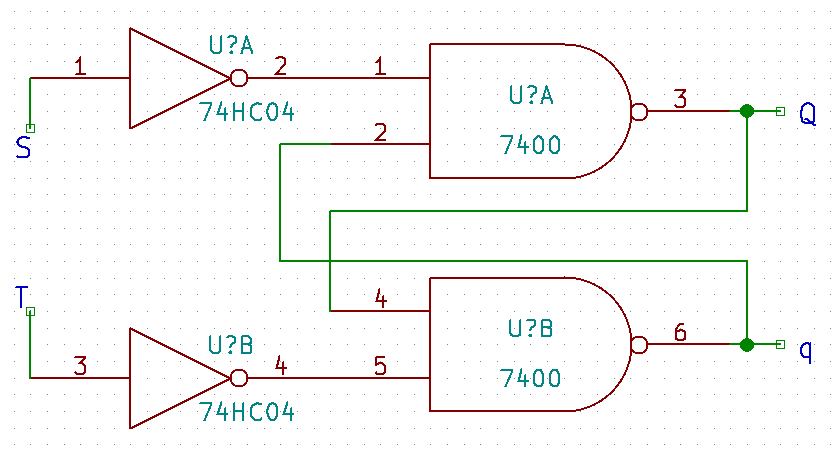
\includegraphics[width=5in]{SR-async.png}
    \caption{S-R asynchronous circuit diagram}
\end{figure}
\begin{figure}[H]
    \centering
    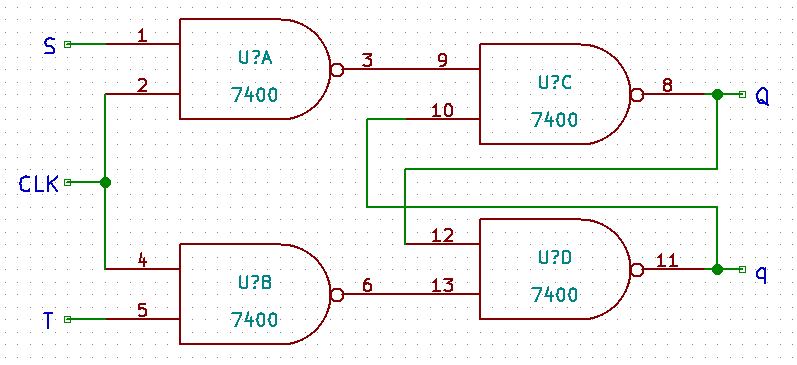
\includegraphics[width=5in]{SR-clocked.png}
    \caption{S-R clocked circuit diagram}
\end{figure}
\begin{figure}[H]
    \centering
    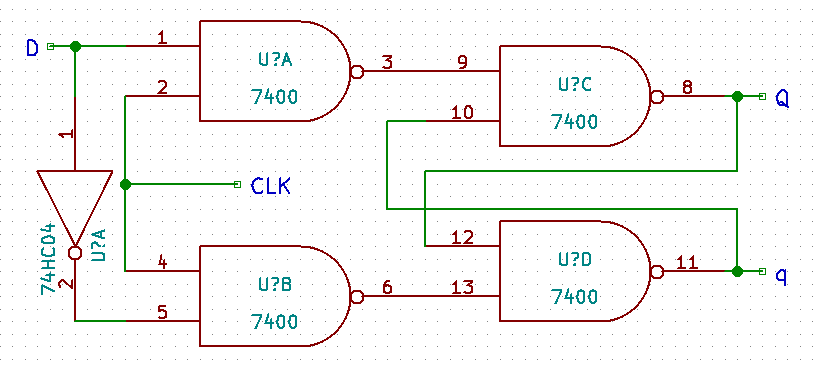
\includegraphics[width=5in]{D-clocked.png}
    \caption{D clocked circuit diagram}
\end{figure}
\begin{figure}[H]
    \centering
    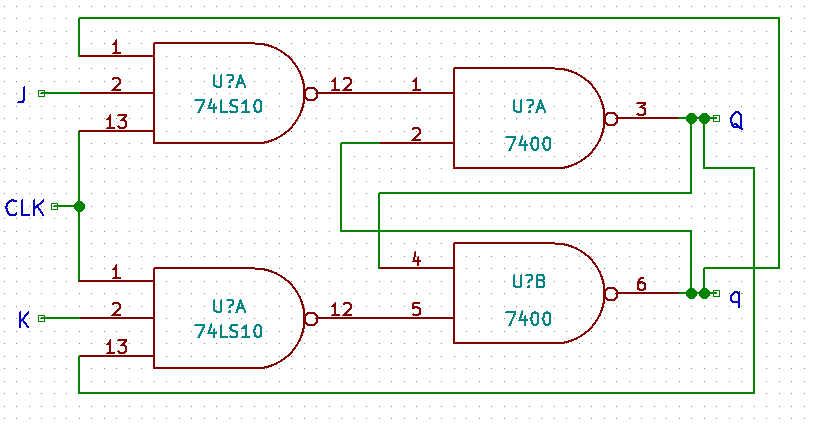
\includegraphics[width=5in]{JK-flipflop.png}
    \caption{J-K flip-flop circuit diagram}
\end{figure}
\begin{figure}[H]
    \centering
    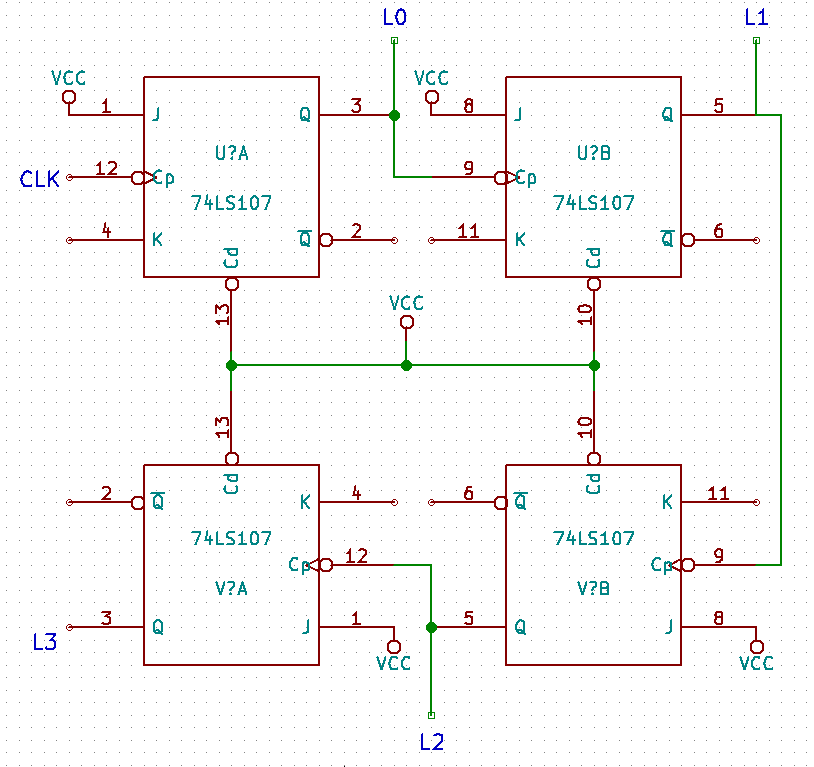
\includegraphics[width=5in]{ripple.png}
    \caption{Binary ripple counter wiring diagram}
\end{figure}
\section{References}
Ronald J. Tocci et al. 2011. Digital Systems: Principles and Applications, 11\textsuperscript{th} Ed.

\end{document}
